% !TeX root = ../main.tex
% 修改稿迁移版：自动编号，原文数据与待核事项保留。
\chapter{团队介绍}
PI OS 项目团队由软件工程、网络安全、人工智能及计算机科学与技术等专业的本科生、硕士生和博士生组成。团队围绕华为“高密部署智能体沙箱引擎”命题，将底层系统研究、工程验证与企业应用需求结合，推进技术实现、实验复核、商业测算和成果转化。

团队成员根据研究与工程经验承担系统研发、智能体机制说明、测试验证、安全分析、财务测算、文档规范和项目统筹等工作，并通过统一术语、数据复核与版本管理保持跨模块协作。

\section{主创团队}\label{sec:8.1}
\subsection{团队构成与能力互补}\label{sec:8.1.1}
项目以运行时扁平化、动态资源卸载和智能内存共享为核心技术方向，目前已完成现阶段核心代码开发。后续重点包括命题指定环境适配、性能与隔离测试、交付文档完善，以及在权属和授权边界明确后推进客户验证。

团队能力可归纳为系统研发与运行时、智能体与卸载机制、测试与安全验证、项目统筹与经营材料四类，形成从技术实现到工程验证、再到商业表达的完整协作链。

\FloatBarrier
\begingroup\linespread{1}\selectfont
\setcounter{table}{0}
\begin{longtable}{@{}>{\raggedright\arraybackslash}p{\dimexpr 0.14062\linewidth-0.5625\tabcolsep\relax}>{\raggedright\arraybackslash}p{\dimexpr 0.30382\linewidth-1.2153\tabcolsep\relax}>{\raggedright\arraybackslash}p{\dimexpr 0.55556\linewidth-2.2222\tabcolsep\relax}@{}}
\caption{PI OS 项目成员与现阶段分工}\label{tab:8-1}\\
\hline
\rowcolor{WordTableHeader} \TableHeaderText{姓名} & \TableHeaderText{年级与专业} & \TableHeaderText{现阶段职责} \\ \hline
\endfirsthead
\multicolumn{3}{c}{\fontsize{9}{12}\selectfont 表 8-1（续）}\\
\hline
\rowcolor{WordTableHeader} \TableHeaderText{姓名} & \TableHeaderText{年级与专业} & \TableHeaderText{现阶段职责} \\ \hline
\endhead
\hline\endfoot\hline\endlastfoot
\rowcolor{WordTableStripe} 
张纪同 & 2023 级本科 · 软件工程 & 项目统筹、命题需求对齐、计划书整合与答辩组织 \\ \hline
陈奕池 & 2026 级博士 · 软件工程 & 核心代码实现、运行时机制研发与技术评审支持 \\ \hline
\rowcolor{WordTableStripe} 
刘国威 & 2024 级博士 · 计算机科学与技术 & 性能优化与技术路线可行性论证支持 \\ \hline
周以恒 & 2026 级硕士 · 计算机科学与技术 & 系统研究、技术文档审核与方案复核支持 \\ \hline
\rowcolor{WordTableStripe} 
范文丽 & 2024 级本科 · 软件工程 & 财务分析与融资计划、团队材料整理与协作证据 \\ \hline
李子鹏 & 2025 级本科 · 计算机科学与技术 & 测试数据复核、指标计算、测试环境与验收材料 \\ \hline
\rowcolor{WordTableStripe} 
刘书雄 & 2024 级本科 · 人工智能 & 智能体任务流程、动态卸载与预取机制说明 \\ \hline
王子硕 & 2025 级本科 · 网络安全 & 隔离与共享安全、数据保护及风险管理材料 \\ \hline
\rowcolor{WordTableStripe} 
王新雅 & 2025 级本科 · 软件工程 & 文档规范、来源整理、术语统一与复现说明 \\ \hline
张思淼 & 2025 级本科 · 软件工程 & 运行时扁平化方案、组件职责与架构说明 \\ \hline
\end{longtable}\endgroup
\par\noindent{\fontsize{9}{13}\selectfont\linespread{1}\selectfont 注：表中职责对应当前项目推进阶段，具体贡献通过代码、测试数据、文档版本和协作记录等材料留存。}

\begin{figure}[H]\centering
\setcounter{figure}{0}
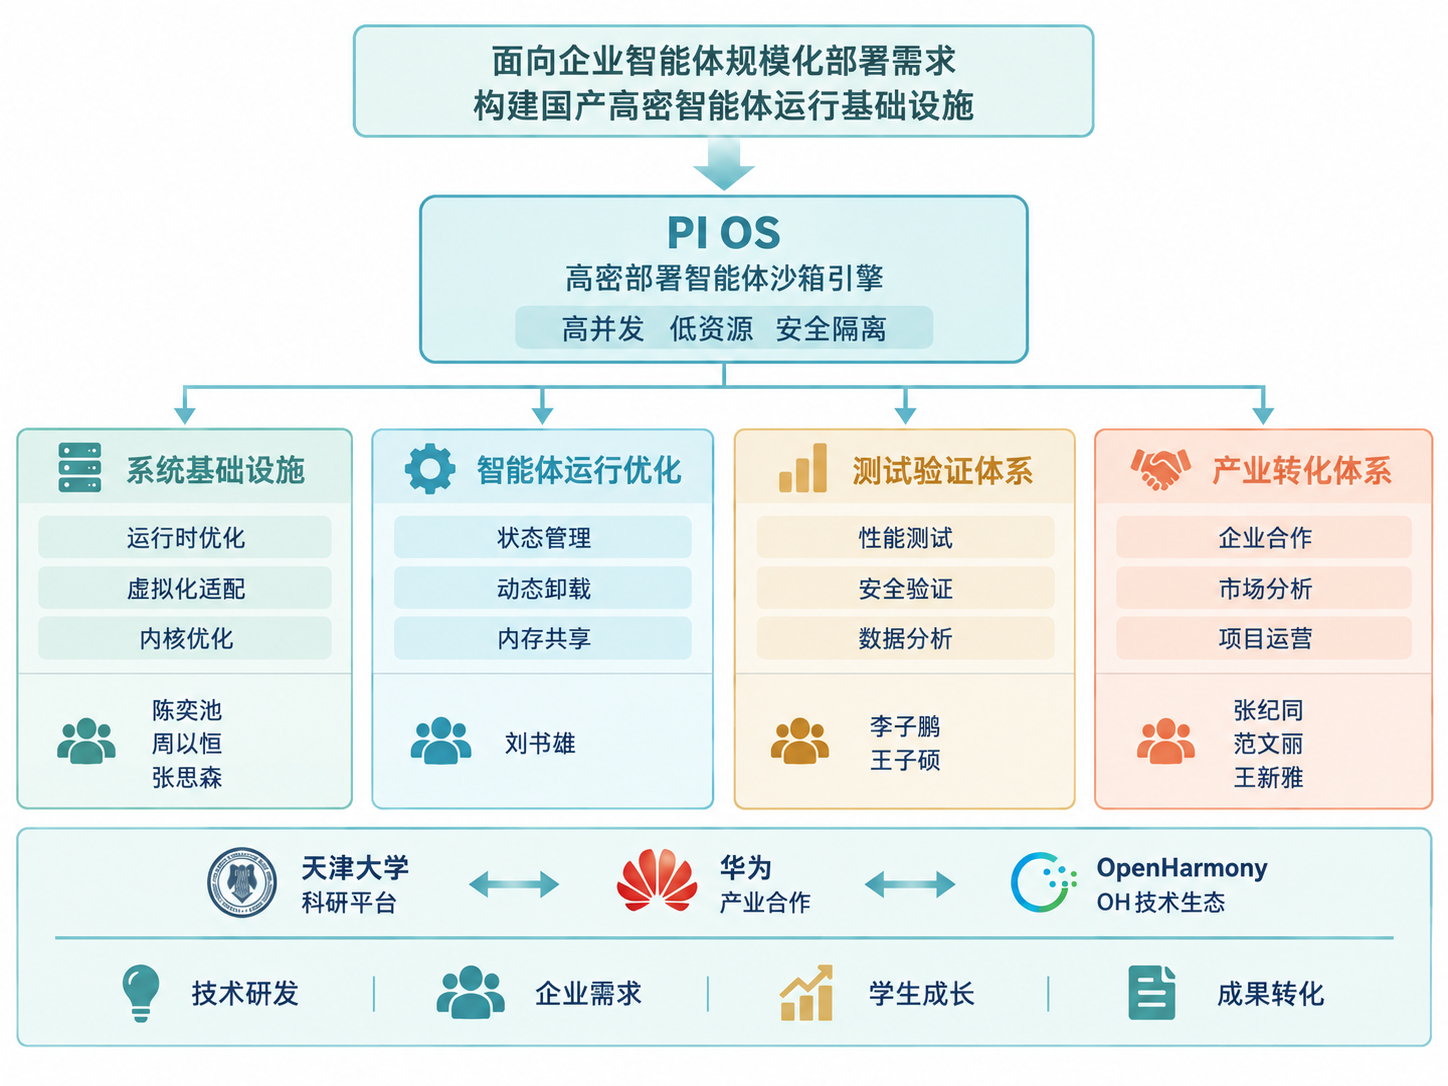
\includegraphics[width=\linewidth,height=.50\textheight,keepaspectratio]{figures/updated-8-1.png}
\caption{团队能力互补结构图}\label{fig:8-1}
\par\vspace{3pt}{\fontsize{9}{12}\selectfont\linespread{1}\selectfont 注：图中分组为所供图稿的工作模块概览；成员学籍、现阶段职责与实际交付物以表 8-1 和表 8-3 为准。}
\end{figure}
\subsection{协作与质量控制机制}\label{sec:8.1.2}
项目采用模块责任制和交叉复核机制。每项核心内容明确主责人、输入材料、结论和复核方式，技术指标保留原始数据、脚本与环境说明，经营数字保留计算依据与关键假设。

\FloatBarrier
\begingroup\linespread{1}\selectfont
\setcounter{table}{1}
\begin{longtable}{@{}>{\raggedright\arraybackslash}p{\dimexpr 0.19531\linewidth-0.7812\tabcolsep\relax}>{\raggedright\arraybackslash}p{\dimexpr 0.61719\linewidth-2.4688\tabcolsep\relax}>{\raggedright\arraybackslash}p{\dimexpr 0.18750\linewidth-0.7500\tabcolsep\relax}@{}}
\caption{团队协作与质量控制机制}\label{tab:8-2}\\
\hline
\rowcolor{WordTableHeader} \TableHeaderText{机制} & \TableHeaderText{执行方式} & \TableHeaderText{作用} \\ \hline
\endfirsthead
\multicolumn{3}{c}{\fontsize{9}{12}\selectfont 表 8-2（续）}\\
\hline
\rowcolor{WordTableHeader} \TableHeaderText{机制} & \TableHeaderText{执行方式} & \TableHeaderText{作用} \\ \hline
\endhead
\hline\endfoot\hline\endlastfoot
\rowcolor{WordTableStripe} 
页面/\allowbreak{}模块责任制 & 每项核心内容明确主责人、输入材料、结论与复核人 & 明确责任边界 \\ \hline
证据留存 & 技术指标保留原始数据、脚本、环境说明和复现步骤；经营数字保留计算依据 & 保证材料可复核 \\ \hline
\rowcolor{WordTableStripe} 
交叉复核 & 技术页由非主责成员检查逻辑和可读性，关键数据至少完成一次独立复算 & 降低单点错误 \\ \hline
统一口径 & 项目名称、技术状态、指标口径、商业化边界在计划书、PPT 和答辩中保持一致 & 提高交付一致性 \\ \hline
\rowcolor{WordTableStripe} 
版本与交接 & 保留代码、测试报告、计划书和展示材料版本；关键模块同步整理部署方法和待办 & 保障项目连续性 \\ \hline
\end{longtable}\endgroup
底层系统开发、工程测试、财务测算和商业表达相互校验：技术结果决定可对外说明的产品能力，测试数据支撑性能与价值判断，财务测算则反向约束人员扩张和客户定价，使技术、市场和财务保持同一套项目口径。

\subsection{学生成长与项目持续性}\label{sec:8.1.3}
团队把企业真实需求转化为可执行的学生实践任务。新成员从环境搭建、测试复现、文档完善和小范围问题修复开始参与，关键修改经评审后合入；个人贡献以任务成果、复核质量和协作记录共同体现。

随着项目进入商业化阶段，团队将根据真实订单和交付负荷补充产品、运维及商务能力。新增岗位以实际工作瓶颈为依据，并通过技术文档、权限交接和备份负责人机制降低人员变化对项目连续性的影响。

\subsection{成员贡献矩阵与成果归属边界}\label{sec:8.1.4}
表 8-1 说明了成员的专业背景与职责分工，表 8-2 说明了协作与质量控制机制。为进一步说明职责对应的实际产出，本节以“成员---实际任务---交付物---证据编号---复核人”的形式列出贡献矩阵，并明确合同核心研发人员、参赛学生与指导教师之间的角色边界与成果归属。

\FloatBarrier
\begingroup\linespread{1}\selectfont
\setcounter{table}{2}
\begin{longtable}{@{}>{\raggedright\arraybackslash}p{\dimexpr 0.10000\linewidth-0.80000\tabcolsep\relax}>{\raggedright\arraybackslash}p{\dimexpr 0.27000\linewidth-2.16000\tabcolsep\relax}>{\raggedright\arraybackslash}p{\dimexpr 0.27000\linewidth-2.16000\tabcolsep\relax}>{\raggedright\arraybackslash}p{\dimexpr 0.25000\linewidth-2.00000\tabcolsep\relax}>{\raggedright\arraybackslash}p{\dimexpr 0.11000\linewidth-0.88000\tabcolsep\relax}@{}}
\caption{PI OS 成员贡献矩阵}\label{tab:8-3}\\
\hline
\rowcolor{WordTableHeader} \TableHeaderText{成员} & \TableHeaderText{实际承担任务} & \TableHeaderText{交付物} & \TableHeaderText{证据编号} & \TableHeaderText{复核人} \\ \hline
\endfirsthead
\multicolumn{5}{c}{\fontsize{9}{12}\selectfont 表 8-3（续）}\\
\hline
\rowcolor{WordTableHeader} \TableHeaderText{成员} & \TableHeaderText{实际承担任务} & \TableHeaderText{交付物} & \TableHeaderText{证据编号} & \TableHeaderText{复核人} \\ \hline
\endhead
\hline\endfoot\hline\endlastfoot
\rowcolor{WordTableStripe} 
张纪同 & 项目统筹、命题需求对齐、计划书整合与答辩组织 & 需求确认与阶段反馈纪要、计划书统稿、答辩材料 & M-01、M-03、V-05 & 周以恒 \\ \hline
陈奕池 & 核心代码实现、运行时机制研发、卸载与预取接口实现 & 接口实现与设计说明、卸载开销对照测试记录 & S-02、V-02、E-04 & 刘国威 \\ \hline
\rowcolor{WordTableStripe} 
刘国威 & 性能优化、技术路线可行性论证 & 性能优化记录、技术路线论证材料 & S-03、E-05 & 陈奕池 \\ \hline
周以恒 & 系统研究、技术文档审核、指标口径统一 & 文档审核记录、指标口径与证据编号规则 & V-03、M-04 & 张纪同 \\ \hline
\rowcolor{WordTableStripe} 
范文丽 & 财务分析与融资计划、团队材料整理与协作证据 & 财务测算表、团队与协作机制材料 & 表 6-1---表 6-5、表 8-1 & 张纪同 \\ \hline
李子鹏 & 测试数据复核、指标计算、测试环境与验收材料 & 测试脚本、并发测试与对照测试记录、环境配置记录 & S-01、E-01、E-06、ENV-01---ENV-03 & 陈奕池 \\ \hline
\rowcolor{WordTableStripe} 
刘书雄 & 智能体任务流程梳理、动态卸载与预取机制说明 & 流程分析材料、资源画像、语义感知实现路径说明 & E-03、图 3-1 与图 3-2 原始材料 & 陈奕池 \\ \hline
王子硕 & 隔离与共享安全、数据保护与风险管理 & 安全边界说明、风险识别与对策材料 & 表 7-1、表 7-2 & 周以恒 \\ \hline
\rowcolor{WordTableStripe} 
王新雅 & 文档规范、来源整理、术语统一与复现说明 & 术语对照表、来源清单、复现说明 & V-04、S-05 & 周以恒 \\ \hline
张思淼 & 运行时扁平化方案、组件职责与架构说明 & 架构说明与组件职责表、架构图原始文件 & V-02、图 3-4 原始材料 & 刘国威 \\ \hline
\end{longtable}\endgroup
\par\noindent{\fontsize{9}{13}\selectfont\linespread{1}\selectfont 注：表中每位成员至少对应一项可独立核对的交付物；同一成员可承担多项任务，交付物由责任人提交、复核人确认后归档。表中未列出的辅助工作（如资料检索、会议记录整理）以纪要或活动记录形式留存。证据编号规则见第 2.8.4 节。}

\FloatBarrier
\begingroup\linespread{1}\selectfont
\setcounter{table}{3}
\begin{longtable}{@{}>{\raggedright\arraybackslash}p{\dimexpr 0.16276\linewidth-0.9766\tabcolsep\relax}>{\raggedright\arraybackslash}p{\dimexpr 0.20616\linewidth-1.2370\tabcolsep\relax}>{\raggedright\arraybackslash}p{\dimexpr 0.22786\linewidth-1.3672\tabcolsep\relax}>{\raggedright\arraybackslash}p{\dimexpr 0.40321\linewidth-2.4193\tabcolsep\relax}@{}}
\caption{项目角色与成果归属边界说明}\label{tab:8-4}\\
\hline
\rowcolor{WordTableHeader} \TableHeaderText{角色类型} & \TableHeaderText{组成} & \TableHeaderText{在项目中的职责} & \TableHeaderText{成果归属与使用边界} \\ \hline
\endfirsthead
\multicolumn{4}{c}{\fontsize{9}{12}\selectfont 表 8-4（续）}\\
\hline
\rowcolor{WordTableHeader} \TableHeaderText{角色类型} & \TableHeaderText{组成} & \TableHeaderText{在项目中的职责} & \TableHeaderText{成果归属与使用边界} \\ \hline
\endhead
\hline\endfoot\hline\endlastfoot
\rowcolor{WordTableStripe} 
合同核心研发人员 & 合作协议中列明的研发人员 & 承担校企科研合作协议约定的研究任务 & 相关成果的使用与公开须遵循天津大学与华为的协议约定，本计划书所述内容以已确认的授权范围为准 \\ \hline
参赛学生团队 & 表 8-1 所列 10 名成员 & 承担方案分析、代码实现、实验复核、财务测算与材料整理等具体工作 & 学生的实际贡献以表 8-3 的交付物与证据编号为依据，与合同之外的团队其他项目成果相互区分 \\ \hline
\rowcolor{WordTableStripe} 
指导教师 & 天津大学赵来平教授 & 负责技术路线、实验方法与关键问题把关 & 指导教师在相关领域的研究积累为项目提供方法支持，不作为 PI OS 的学生交付成果计入 \\ \hline
导师团队其他合作项目成果 & 华为 FunctionGraph 应用证明、腾讯 UNMOOR 应用证明等 & 反映团队在相关技术方向的产业验证经历 & 属于相关技术方向的产业应用与技术积累证据，不等同于 PI OS 已在这些平台落地，不作为本项目的客户或收入证明 \\ \hline
\end{longtable}\endgroup
上述边界说明与本计划书“证明材料”部分的材料边界说明保持一致。项目在对外展示与答辩中统一使用同一口径：合同阶段完成不等于产品最终验收完成，相关技术积累不等于本项目已实现商业化落地。

图 8-2 呈现成员贡献、证据编号与复核关系；图 8-3 呈现不同角色在成果归属上的边界。

\begin{figure}[H]\centering
\setcounter{figure}{1}
\begin{tikzpicture}[x=1cm,y=.78cm, every node/.style={font=\fontsize{9}{12}\selectfont\linespread{1}\selectfont,align=center},box/.style={draw=DiagramRule,rounded corners=2pt,fill=DiagramLight,inner sep=4pt},arr/.style={->,>=stealth,thick,draw=DiagramMain}]
\node[box,text width=1.5cm,fill=DiagramMain,text=white] (a) at (1,0) {成员};
\node[box,text width=6.6cm,fill=DiagramMain,text=white] (b) at (6,0) {交付物与证据编号};
\node[box,text width=1.8cm,fill=DiagramMain,text=white] (c) at (11.4,0) {复核人};
\node[box,text width=1.5cm,minimum height=.78cm] (a0) at (1,-1.1) {张纪同};
\node[box,text width=6.6cm,minimum height=.78cm] (b0) at (6,-1.1) {M-01、M-03、V-05};
\node[box,text width=1.8cm,minimum height=.78cm] (c0) at (11.4,-1.1) {周以恒};
\draw[arr] (a0) -- (b0);\draw[arr] (b0) -- (c0);
\node[box,text width=1.5cm,minimum height=.78cm] (a1) at (1,-2.18) {陈奕池};
\node[box,text width=6.6cm,minimum height=.78cm] (b1) at (6,-2.18) {S-02、V-02、E-04};
\node[box,text width=1.8cm,minimum height=.78cm] (c1) at (11.4,-2.18) {刘国威};
\draw[arr] (a1) -- (b1);\draw[arr] (b1) -- (c1);
\node[box,text width=1.5cm,minimum height=.78cm] (a2) at (1,-3.2600000000000002) {刘国威};
\node[box,text width=6.6cm,minimum height=.78cm] (b2) at (6,-3.2600000000000002) {S-03、E-05};
\node[box,text width=1.8cm,minimum height=.78cm] (c2) at (11.4,-3.2600000000000002) {陈奕池};
\draw[arr] (a2) -- (b2);\draw[arr] (b2) -- (c2);
\node[box,text width=1.5cm,minimum height=.78cm] (a3) at (1,-4.34) {周以恒};
\node[box,text width=6.6cm,minimum height=.78cm] (b3) at (6,-4.34) {V-03、M-04};
\node[box,text width=1.8cm,minimum height=.78cm] (c3) at (11.4,-4.34) {张纪同};
\draw[arr] (a3) -- (b3);\draw[arr] (b3) -- (c3);
\node[box,text width=1.5cm,minimum height=.78cm] (a4) at (1,-5.42) {范文丽};
\node[box,text width=6.6cm,minimum height=.78cm] (b4) at (6,-5.42) {表 6-1---表 6-5、表 8-1};
\node[box,text width=1.8cm,minimum height=.78cm] (c4) at (11.4,-5.42) {张纪同};
\draw[arr] (a4) -- (b4);\draw[arr] (b4) -- (c4);
\node[box,text width=1.5cm,minimum height=.78cm] (a5) at (1,-6.5) {李子鹏};
\node[box,text width=6.6cm,minimum height=.78cm] (b5) at (6,-6.5) {S-01、E-01、E-06、ENV-01---ENV-03};
\node[box,text width=1.8cm,minimum height=.78cm] (c5) at (11.4,-6.5) {陈奕池};
\draw[arr] (a5) -- (b5);\draw[arr] (b5) -- (c5);
\node[box,text width=1.5cm,minimum height=.78cm] (a6) at (1,-7.58) {刘书雄};
\node[box,text width=6.6cm,minimum height=.78cm] (b6) at (6,-7.58) {E-03、图 3-1 与图 3-2 原始材料};
\node[box,text width=1.8cm,minimum height=.78cm] (c6) at (11.4,-7.58) {陈奕池};
\draw[arr] (a6) -- (b6);\draw[arr] (b6) -- (c6);
\node[box,text width=1.5cm,minimum height=.78cm] (a7) at (1,-8.66) {王子硕};
\node[box,text width=6.6cm,minimum height=.78cm] (b7) at (6,-8.66) {表 7-1、表 7-2};
\node[box,text width=1.8cm,minimum height=.78cm] (c7) at (11.4,-8.66) {周以恒};
\draw[arr] (a7) -- (b7);\draw[arr] (b7) -- (c7);
\node[box,text width=1.5cm,minimum height=.78cm] (a8) at (1,-9.74) {王新雅};
\node[box,text width=6.6cm,minimum height=.78cm] (b8) at (6,-9.74) {V-04、S-05};
\node[box,text width=1.8cm,minimum height=.78cm] (c8) at (11.4,-9.74) {周以恒};
\draw[arr] (a8) -- (b8);\draw[arr] (b8) -- (c8);
\node[box,text width=1.5cm,minimum height=.78cm] (a9) at (1,-10.82) {张思淼};
\node[box,text width=6.6cm,minimum height=.78cm] (b9) at (6,-10.82) {V-02、图 3-4 原始材料};
\node[box,text width=1.8cm,minimum height=.78cm] (c9) at (11.4,-10.82) {刘国威};
\draw[arr] (a9) -- (b9);\draw[arr] (b9) -- (c9);
\end{tikzpicture}
\caption{成员贡献、证据编号与复核关系图}\label{fig:8-2}
\end{figure}
\begin{figure}[H]\centering
\setcounter{figure}{2}
\begin{tikzpicture}[x=1cm,y=.82cm, every node/.style={font=\fontsize{9}{12}\selectfont\linespread{1}\selectfont,align=center},box/.style={draw=DiagramRule,rounded corners=2pt,fill=DiagramLight,inner sep=6pt},arr/.style={->,>=stealth,thick,draw=DiagramMain}]
\node[box,text width=11.7cm,fill=DiagramMain,text=white] (p) at (6.5,0) {\textbf{PI OS 直接项目证据}\\合作协议、阶段测试报告、代码与文档记录、实验脚本与复现说明};
\node[box,text width=11.7cm,] (t) at (6.5,-1.9) {\textbf{相关技术积累证据}\\华为 FunctionGraph 应用证明、腾讯 UNMOOR 应用证明\\反映相关方向经历，不作为 PI OS 客户、收入或平台落地证明};
\node[box,text width=11.7cm,dashed] (auth) at (6.5,-4.1) {\textbf{成果使用与公开边界}\\合同核心研发人员：遵循校企合作协议\\参赛学生：以具体交付物与表 8-3 记录认定贡献\\指导教师：技术路线与方法指导，研究积累不计入学生交付成果};
\node[box,text width=11.7cm,] (note) at (6.5,-6.4) {已完成：核心代码与研究环境测试；正在验证：指定环境适配；后续计划：授权后交付与试点。};
\end{tikzpicture}
\caption{项目角色与成果归属边界图}\label{fig:8-3}
\end{figure}
\section{指导教师}\label{sec:8.2}
本项目指导教师为天津大学赵来平教授。赵来平教授研究领域为计算系统，研究方向包括数据中心、云计算、软件定义网络和智能运维，主讲云计算课程并承担研究生指导工作，其研究方向与 PI OS 涉及的智能体运行环境、计算资源管理和系统运行效率优化具有较高相关性。

项目推进过程中，指导教师主要负责技术路线、实验方法和关键问题把关，具体的方案分析、代码实现、实验复核、财务测算和材料整理由团队成员按分工完成。该协作方式既保证技术方向和实验方法的规范性，也保留学生团队在项目实现与交付中的主体作用。

